
\documentclass{article}
\usepackage{tikz}
\begin{document}
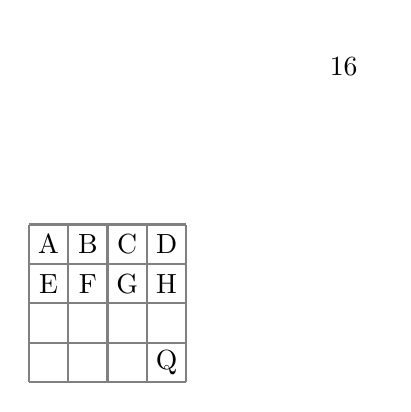
\begin{tikzpicture}[thick]  
\draw[step=0.5cm,color=gray] (-1,-1) grid (1,1);
\node at (-0.75,+0.75) {A};
\node at (-0.25,+0.75) {B};
\node at (+0.25,+0.75) {C};
\node at (+0.75,+0.75) {D};
\node at (-0.75,+0.25) {E};
\node at (-0.25,+0.25) {F};
\node at (+0.25,+0.25) {G};
\node at (+0.75,+0.25) {H};
% ...
\node at (+0.75,-0.75) {Q};
\node[fill=white!20, minimum size=1cm, inner sep=0pt] at (3,3) {$16$};

  

\end{tikzpicture}

\end{document}
    